%!TEX root = iclr2026_conference.tex
\begin{figure}[t]
  \centering
  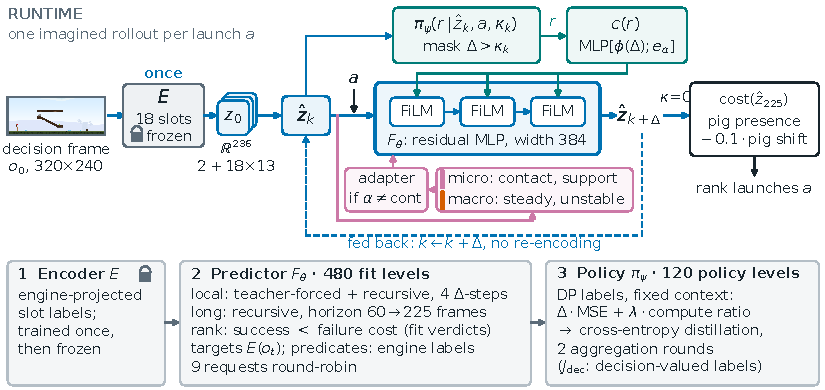
\includegraphics[width=\linewidth]{fig_model_overview_rev}
  \caption[Primary model]{\rev{\textbf{Primary model.} Top, runtime: $E$ parses only the decision frame $o_0$. At each step $\pi_\psi$ picks $r=(\Delta,\alpha)$, $c(r)$ modulates the shared predictor $F_\theta$, and a predicate head feeds back only when $\alpha\neq\textsf{cont}$. Predictions are fed back without re-encoding until $\kappa=0$, and the tie-free cost (Equation~\ref{eq:taskcost}) ranks launches. Bottom, training: $E$ on engine labels, then frozen; $F_\theta$ on predictor-fit levels, with a ranking loss on their outcomes; $\pi_\psi$ distilled from DP labels (Equation~\ref{eq:objective}) on policy-fit levels. Live evaluation restarts the level for each shot.}}
  \label{fig:mth:arch}
\end{figure}
